\documentclass{acm_proc_article-sp}
\usepackage[utf8]{inputenc}
\usepackage{epstopdf}
\usepackage{times}
\usepackage{natbib}
\usepackage{amsmath}
\usepackage{dcolumn}
\usepackage{graphicx}
\usepackage{xspace}
\usepackage{color}
\usepackage{listings}
\usepackage{float}
%\usepackage{amsmath, amsthm, amssymb, amsfonts}
%\usepackage{tabularx}
\usepackage{array}
%\usepackage{tabulary}%can use align in tables with line breaks
\usepackage{multirow}
\usepackage{rotating,makecell}
\usepackage{booktabs} %adds new commands toprule midrule and bottomrule for professionally looking tables

\usepackage[breaklinks=true, bookmarksopen=true,bookmarksnumbered=true]{hyperref}
\urlstyle{same}
% \usepackage{titling} % To modify the title
%\usepackage[hmargin=1.3in]{geometry}
% \setlength{\droptitle}{-5em}   % This is your set screw


\definecolor{Brown}{cmyk}{0,0.81,1,0.60}
\definecolor{OliveGreen}{cmyk}{0.64,0,0.95,0.40}
\definecolor{CadetBlue}{cmyk}{0.62,0.57,0.23,0}
\definecolor{lightlightgray}{gray}{0.9}

% listing styles
\lstset{
    numberbychapter=false,
    basicstyle=\ttfamily\footnotesize,
    numbers=none,
    captionpos=b,
    frame=single,
    breaklines=true,
    breakatwhitespace,
    columns=fullflexible,
    commentstyle=\itshape\color{OliveGreen},
    keywordstyle=\bfseries\color{CadetBlue}
}


\lstdefinestyle{SPARQL}{
  backgroundcolor=\color{lightlightgray}, % Choose background color
  morecomment=[l]{\#},
  morekeywords={SELECT, CONSTRUCT, FROM, WHERE, FILTER, GROUP BY, IN, AS,
    LIMIT,OFFSET,PREFIX,OPTIONAL,UNION,NOT,EXISTS,AVG,BIND,
    obs,foaf,rdf,skos,rdfs,ex,xsd,owl,skosxl,doap,void,dbo,earl,cex,qb}
 }

\lstdefinestyle{Turtle}{
  backgroundcolor=\color{lightlightgray}, % Choose background color
  morecomment=[l]{\#},
  morekeywords={@PREFIX,BASE,a,foaf, @prefix, rdf,
    obs,qb,cex,skos, skosxl, rdf, rdfs, ex, xsd, wr,
    wt,dc,lemon,doap,void,dbo,owl}
 }
    
\lstdefinestyle{Turtle}{numberblanklines=true, morekeywords={foaf, prefix, rdf,
    skos, skosxl, rdfs, ex, xsd, wr, wt, dc, lemon, doap, doap,void, dbo, owl,
    @prefix}}


%\usepackage{textcomp}
\lstdefinestyle{XML}
{
  morestring=[b]",
  morestring=[s]{>}{<},
  morecomment=[s]{<?}{?>},
  stringstyle=\color{black},
  identifierstyle=\color{darkblue},
  keywordstyle=\color{cyan},
  morekeywords={xmlns,version,type}% list your attributes here
}

\sloppy

%%%%%%%%%%% Put your definitions here


%%%%%%%%%%% End of definitions

\newcommand{\TODO}[1]{{\color{red}{\textbf{TODO: {#1}}\xspace}}}
\newcommand{\todo}[1]{{\TODO{{#1}}}}

\newcommand{\CONSIDER}[1]{{\color{blue}{\textbf{CONSIDER: {#1}}\xspace}}}
   
\newcommand{\desc}{\noindent\emph{Description:}}

\newcommand{\footnoteUrl}[1]{\footnote{\url{#1}}}

\newcolumntype{d}[1]{D{.}{.}{#1}}

\floatplacement{figure}{H}

\begin{document}

\title{Representing verifiable statistical index computations as linked data}

\numberofauthors{2} 
\author{
\alignauthor
Jose Emilio Labra Gayo\\
       \affaddr{University of Oviedo}\\
       \affaddr{Dept. of Computer Science}\\
       \affaddr{C/Calvo Sotelo, S/N}\\
       \email{labra@uniovi.es}
\alignauthor
Hania Farham\\
       \affaddr{The Web Foundation}\\
       \email{hania@webfoundation.org}
\and
\alignauthor
Juan Castro Fernández\\
       \affaddr{WESO Research Group} \\
       \affaddr{University of Oviedo}\\
       \affaddr{C/Calvo Sotelo, S/N}\\
       \email{juan.castro@weso.es}
\alignauthor
Jose María Álvarez Rodríguez\\
       \affaddr{Dept. Computer Science} \\
       \affaddr{Carlos III University}\\
       \affaddr{Leganés, Madrid}\\
       \email{josemaria.alvarez@uc3m.es}
}

\maketitle
\begin{abstract}

In this paper we describe the development of the Web Index linked data portal that represents statistical index data and computations. 

The Web Index is a multi-dimensional measure of the World Wide Web’s contribution to development and human rights globally. It covers 81 countries and incorporates indicators that assess several areas like universal access; freedom and openness; relevant content; and empowerment.

In order to empower the Web Index transparency, one internal requirement was that every published data could be externally verified. 
The verification could be that it was just raw data obtained from an external source, in which case, the system must provide a link to the data source or that the value has been internally computed, 
 in which case, the system provides links to those values.
The resulting portal contains data that can be tracked to its sources so an external agent
can validate the whole index computation process.

We describe the different aspects on the development of the WebIndex data portal, which also offers new linked data visualization tools. 

Although in this paper we concentrate on the Web Index development, 
we consider that this approach can be generalized to other projects which involve 
 the publication of externally verifiable statistical computations.
\end{abstract}

% A category with the (minimum) three required fields
\category{H.2.8}{Database Applications}{Statistical databases}
%A category including the fourth, optional field follows...
\category{H.3.5}{Online Information Services}{Web-based services}

\terms{Theory}

\keywords{Linked data, Statistics, Computations, RDF} 

\section{Introduction}

The creation and use of quantitative indexes is a widely 
accepted practice that has been applied to numerous domains like economics and
Bibliometrics (Impact factor), 
research and academic performance (H-Index or Shanghai rankings), 
 cloud computing (Global Cloud Index, by CISCO), 
etc.

We consider that those indexes could benefit from a 
 Linked Data approach where the rankings could be seen, tracked and 
 verified by their users.

We participated in the Web Index project
(\url{http://thewebindex.org}), which created an index to measure the Web impact in different countries.

The 2012 version offered a data
portal\footnoteUrl{http://data.webfoundation.org} whose data was obtained 
by transforming raw observations and precomputed values 
from Excel sheets to RDF~\cite{Alvarez13}. 

In the 2013 version of that data portal, we are working on 
both validating and computing observations to automatically generate the index from raw data.

We have defined a generic vocabulary 
of computational index structures which could be applied to compute and validate any other kind of index and can be seen as an specialization of the RDF Data Cube vocabulary~\cite{Cube}.

The validation process employs a combination of SPARQL~\cite{SPARQL11} queries and Shape Expressions \cite{Boneva2014} to check the 
 different integrity constraints and computation steps in a declarative way.

Given that the most important part of a data portal about statistical indexes are the 
numeric values of each observations we established the internal requirement that any value published should be justified either declaring from where it had been obtained or
linking it to the values of other observations
from which it had been computed.

The resulting data portal \url{http://data.webfoundation.org/webindex/2013} contains not only a linked data view about
the statistical data but also a machine verifiable justification of the index ranks.

%At this moment, we have a running example and a validator which 
% reads and executes the SPARQL queries. 
% Source code and some examples are available
% at~\url{https://github.com/weso/computex}. 
% Although our prototype validator has been implemented in Scala, 
% our approach is independent of any programming language 
% as far as it can load and execute SPARQL 1.1 queries.

Along the paper we will use Turtle and SPARQL notation and assume that the
namespaces have been declared using the most common prefixes found in
\url{http://prefix.cc}.

\section{WebIndex Computation Process}

The Web Index is a composite measure that summarizes in a single (average) number the impact and value derived from the Web in various countries. There are serious challenges when attempting to measure and quantify some of the dimensions the Index covers (e.g. the social and political), and suitable proxies were used instead.

As the Web Index covers a large number of countries, some of which have serious data deficiencies or were not covered by the data providers, we needed to impute the missing data. 
A number of experts in the relevant fields were selected to overcome these challenges and 
produce a robust and rigorous Index.

Two types of data were used in the construction of the Index: existing data from other data providers (\emph{secondary data}), and new data gathered via a multi-country questionnaire (\emph{primary data}) 
that was specifically designed by the Web Foundation and its advisers. 
These primary data will begin to fill in some of the gaps in measurement of the utility and impact of the Web in various countries. 
Indeed, the data gaps in this field are significant, and we aim to expand those questionnaires in future editions of the Index, both in terms of the questions/indicators gathered and the number of countries covered by the Index.

There are several steps in the process of constructing a composite Index. Some of those involve deciding which statistical method to use in the normalisation and aggregation processes. In arriving at that decision, we took into account several factors, including the purpose of the Index, the number of dimensions we were
aggregating, and the ease of disseminating and communicating it, in an understandable, replicable and transparent way. The following 10 steps summarise the computation process of the Index:

\begin{enumerate}

\item Take the data for each indicator from the data source for the 81 countries covered by the Index for the 2007-2012 time period (or 2013, in the case of the Web Index expert assessment survey).

\item Impute missing data for every secondary indicator for the sample of 81 countries over the period 2007-2012. Some indicators were not imputed as it was not logical to do so. None of the primary data indicators were imputed. Hence the 2013 Index is very different from the 2007-2012 Indexes that were computed using secondary data only.

Broadly, the imputation of missing data was done using two methods: country-mean substitution if the missing number is in the middle year (e.g. have 2008 and 2010 but not 2009), or taking arithmetic growth rates on a year-by-year basis. Most missing data for 2011 and 2012 are imputed by applying the arithmetic growth rate for the period, to the 2010 number. For the indicators that did not cover a particular country in any of the years, no imputation was done for that country/indicator.

\item Normalise the full (imputed) dataset using z-scores, making sure that for all indicators, a high value is \emph{good} and a low value is \emph{bad}.

\item Cluster some of the variables (as per the scheme in the tree diagram), taking the average of the clustered indicators post normalisation. For the clustered indicators, this clustered value is the one to be used in the computation of the Index components.

\item Compute the nine component scores using arithmetic means, 
 using the clustered values where relevant.

\item Compute the min-max values for each z-score value of the components, 
 as this is what will be shown in the visualisation tool and other 
 publications containing the component values (generally, it is easier to understand 
 a min-max number in the range of 0 – 100 rather than a standard deviation-based number). 
 The formula for this is: $\frac{x-min}{max-min}\times{}100$

\item Compute sub-index scores by calculating the weighted averages of the relevant components for each sub-Index.

\item Compute the min-max values for each z-score value of the sub-Indexes, as this is what will be shown in the visualization tool and other publications containing the sub-index values.

\item Compute overall composite scores by calculating the weighted average of the sub-indexes.

\item Compute the min-max values (on a scale of 0-100) for each z-score value of the overall composite scores, as this is what will be shown in the visualisation tool and other publications containing the composite scores.
\end{enumerate}

The computation process was originally done by human experts using the Excel file although
once the process was established, we considered that it could be automated so we
could validate the whole process. 

\section{WebIndex workflow}

The WebIndex workflow has been depicted in figure~\ref{Fig:WebIndexWorkFlow}. 

The Excel file was comprised of 184 Excel sheets and contained a combination
 of raw, imputed and normalized data created by human experts using Excel. 

That external data filtered and converted to RDF by means of an specialized web service called \emph{wiFetcher}. 

Although some of the imported values had been
 pre-computed in Excel by human experts, we collected only the raw values, so we could validate the computation process. 

In this way, another application called \emph{wiCompute} took the raw values and computed the index following the
computation steps defined by the experts. 
\emph{wiCompute} carried out the computations
 generating RDF datasets for the intermediary results and linking the generated values
 to the values from which they had been computed.
 
Finally, the RDF data generated was published to a SPARQL endpoint from which we created
a specialized visualization tool called \emph{Wesby}.

\begin{figure*}[h]
\begin{center}
  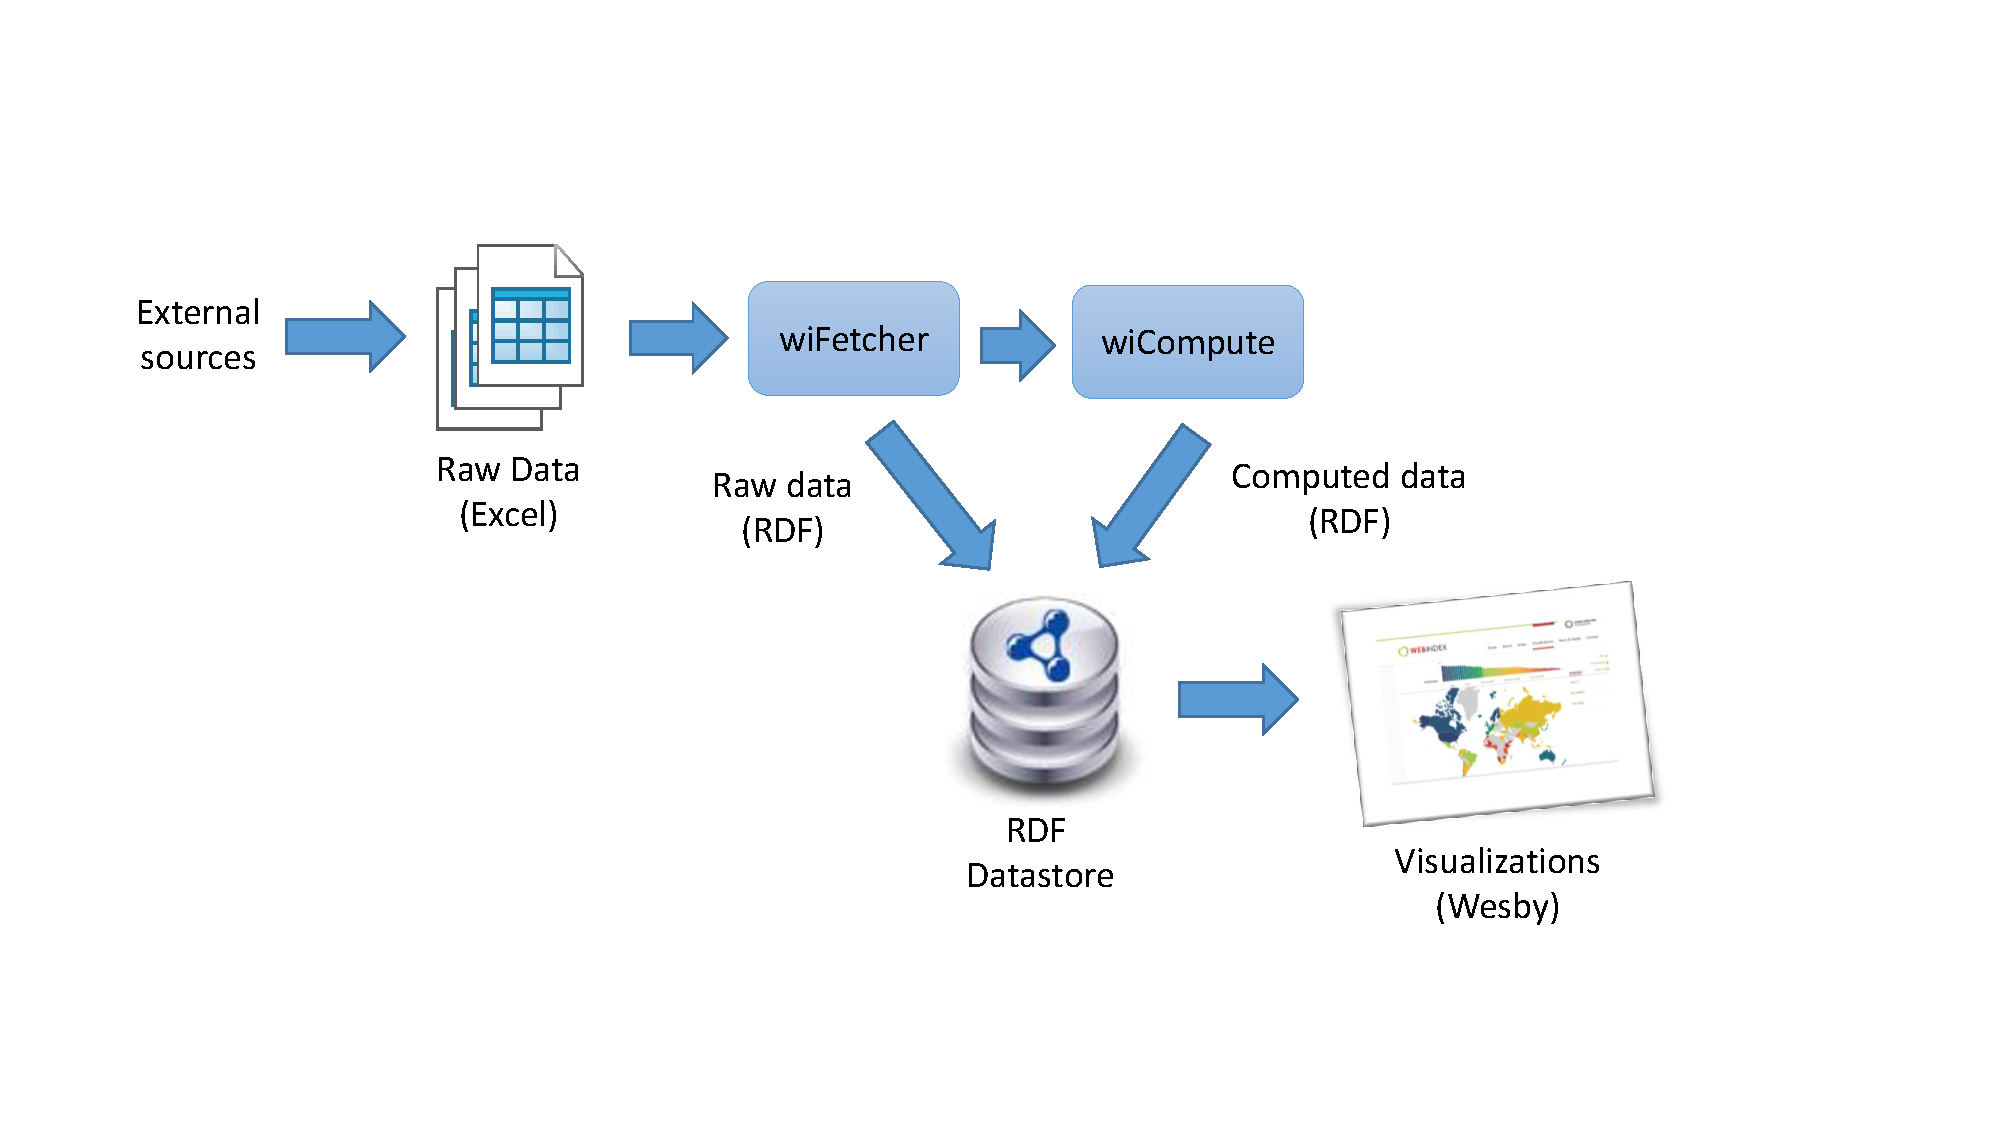
\includegraphics[width=0.9\textwidth]{WebIndexWorkFlow}
\end{center}
\caption{Web Index data portal WorkFlow}
\label{Fig:WebIndexWorkFlow}
\end{figure*}


\section{WebIndex data portal representation}

Given the statistical nature of the data, we opted by reusing the RDF Data Cube vocabulary. 
  
Our data model consists of a list of observations which can be raw observations
obtained from an external source or computed observations derived from other
observations. 
An example observation can be:

\begin{lstlisting}[style=SPARQL]
obs:obsM23 a qb:Observation ;
 cex:computation [ a cex:Z-Score ; 
      cex:observation obs:obsA23 ; cex:slice slice:sliceA09 ; ] ;
 cex:value 0.56 ;
 cex:md5-checksum "2917835203..." ;
 cex:indicator indicator:A ;
 cex:concept country:ESP ;
 qb:dataSet dataset:A-Normalized ;
 # ... other declarations omitted for brevity
\end{lstlisting}

Where we declare that \lstinline|obs:obsM23| is an observation
 whose value is \lstinline|0.56| that has been obtained as the Z-Score
 of the observation \lstinline|obs:A23| using the slice
 \lstinline|slice:sliceA09|. The observations refers to indicator
 \lstinline|indicator:A|, to the concept \lstinline|country:ESP| and to the
 dataset \lstinline|dataset:A-Normalized|.
 
For each observation, we also add a value for 
\lstinline|cex:md5-checksum| which is obtained as a combination of the 
different values of the observation and allows a user to verify the
values asserted to that observation.


\section{Computex vocabulary}

The \emph{Computex} vocabulary is available
at~\url{http://purl.org/weso/computex}. It defines terms related to the
computation of statistical index data and is compatible with RDF Data Cube
vocabulary. Some terms defined in the vocabulary are:

\begin{itemize}
\item\textbf{\lstinline|cex:Concept|} represents the entities that we are
indexing.
In the case of the Web Index project, the concepts are the different countries.
In other applications it could be Universities, journals, services, etc.

\item\textbf{\lstinline|cex:Indicator|}. A dimension whose values add
information to the Index.
Indicators can be simple dimensions, for example: the mobile phone
suscriptions per 100 population, or can be composed from other
indicators. 

\item\textbf{\lstinline|qb:Observation|}. This is the same term as in the 
RDF Data Cube vocabulary. It contains values for the
properties: \lstinline|cex:value|, \lstinline|cex:indicator| 
and \lstinline|cex:concept|, etc. 
The value of a \lstinline|qb:Observation| can be a Raw value
   obtained from an external source or a computed value obtained from other
   observations.

\item\textbf{\lstinline|cex:Computation|}. We have declared the main computation
types that we needed for the WebIndex project, which have been summarized in
Table~\ref{table:computations}. That list of computation types is non-exhaustive
and can be further extended in the future. 

\item\textbf{\lstinline|cex:WeightSchema|} a weight schema for a list of
indicators. It consists of a weight associated for each indicator which can be
used to compute an aggregated observation.

\end{itemize}

\begin{table*}[t]
\label{table:computations}
\begin{center}
\begin{tabular}{ p{0.2\textwidth} p{0.5\textwidth} p{0.3\textwidth}}
\toprule
Computation & Description & Properties \\
\hline
Raw			& No computation. Raw value obtained from external source.
			&  \\
Mean	    & Mean of a set of observations 
			& \lstinline|cex:observation| \newline 
			  \lstinline|cex:slice| \\
Increment	& Increment an observation by a given amount 
			& \lstinline|cex:observation| \newline 
			  \lstinline|cex:amount|  \\
Copy		& A copy of another observation 
			& \lstinline|cex:observation| \\
Z-score		& A normalization of an observation using the values from a Slice. 
			& \lstinline|cex:observation| \newline 
			  \lstinline|cex:slice| \\
Ranking		& Position in the ranking of a slice of observations. 
			& \lstinline|cex:observation| \newline 
			  \lstinline|cex:slice| \\
AverageGrowth & Expected average growth of N observations
			  & \lstinline|cex:observations| \\
WeightedMean & Weighted mean of an observation
			& \lstinline|cex:observation| \newline
			  \lstinline|cex:slice|       \newline
			  \lstinline|cex:weightSchema| \\
\bottomrule\\
\end{tabular}
\caption{Some types of statistical computations}
\end{center}
\end{table*}

\section{Validation approach}

The validation approach employed in the 2012 WebIndex project was based on
 resource templates similar to the OSLC resource
 shapes\footnoteUrl{http://www.w3.org/2012/12/rdf-val/SOTA} and
 the MD5 checksum field. 
 Apart from that, we did not verify that the precomputed values imported from
 the Excel sheets really match the value that could be obtained by 
 following the declared computation process.

We propose a new validation approach that goes a step forward. 
The goal is not only to check that a resource contains a given set of fields and values, but also that those values really match
the values that can be obtained by following the declared computations.
 
The proposed approach has been inspired by the integrity
constraint specification proposed by the RDF Data Cube vocabulary 
which employs a set of SPARQL
 \lstinline|ASK| queries to check the integrity of RDF Data Cube data. 
 Although \lstinline|ASK| queries provide a good means to check integrity, in
 practice their boolean nature does not offer too much help when a 
 dataset does not accomplish with the data model.

We decided to use \lstinline|CONSTRUCT| queries which, in case of error, 
  contain an error message and a list of error parameters that can help to spot
  the problematic data.

 We transformed the \lstinline|ASK| queries defined in the RDF Data Cube
 specification to \lstinline|CONSTRUCT| queries. For example, the
 query to validate the RDF Data Cube integrity constraint 4 (IC-4) is:
 
\begin{lstlisting}[style=SPARQL]
CONSTRUCT {
 [ a cex:Error ; cex:errorParam [cex:name "dim"; cex:value ?dim ] ;
   cex:msg "Every Dimension must have a declared range" . ]
} WHERE { ?dim a qb:DimensionProperty .
  FILTER NOT EXISTS { ?dim rdfs:range [] }
}
\end{lstlisting}
 
In order to make our error messages compatible with EARL~\cite{EARL}, we have
 defined \lstinline|cex:Error| as a subclass of \lstinline|earl:TestResult| and 
 declared it to have the value \lstinline|earl:failed| for the property
 \lstinline|earl:outcome|.
 
We have also created our own set of SPARQL \lstinline|CONSTRUCT| queries to
validate the \emph{Computex} vocabulary terms, specially the computation of index data.
For example, the following query validates that every observation 
  has at most one value.
 
\begin{lstlisting}[style=SPARQL]
CONSTRUCT {
 [ a cex:Error ; cex:errorParam  # ... omitted 
    cex:msg "Observation has two different values" . ]
} WHERE { ?obs a qb:Observation . 
 ?obs cex:value ?value1 . ?obs cex:value ?value2 .
 FILTER ( ?value1 != ?value2  )
}
\end{lstlisting}

Using this approach, it is possible to define more expressive validations.
For example, we are able to validate that an observation has been obtained as
the mean of other observations. 

\begin{lstlisting}[style=SPARQL]
CONSTRUCT {
 [ a cex:Error ; cex:errorParam # ...omitted 
   cex:msg "Mean value does not match" ] . 
} WHERE { 
    ?obs a qb:Observation ;
         cex:computation ?comp ;
         cex:value ?val .
  ?comp a cex:Mean .
  { SELECT (AVG(?value) as ?mean) ?comp WHERE {
     ?comp cex:observation ?obs1 .
	 ?obs1 cex:value ?value ;
  } GROUP BY ?comp } 
 FILTER( abs(?mean - ?val) > 0.0001)
}
\end{lstlisting}

We have implemented an online validation tool called \emph{Computex}\footnote{\url{http://computex.herokuapp.com/}} which takes as
 input an RDF graph and checks if it follows the integrity constraints defined by Computex.
 The validation tool can also check if the RDF graph follows the RDF Data Cube integrity constraints
 and it can also do the index computation for RDF Graphs. 
 Although this declarative approach was very elegant, computing the webindex using only SPARQL queries
 was not practical (it took around 15 minutes for a small subset), so the computation process was finally done
 by a specialized program implemented in Scala~\footnote{Source code is available here: \url{https://github.com/weso/wiCompute}}. 
  
\section{Expressiveness limits of SPARQL queries}

Validating statistical computations using SPARQL queries offered 
 a good exercise to check SPARQL expressivity. Although we were able 
 to express most of the computation types, some of them had to employ functions
 that are not part of SPARQL 1.1 or had to be defined in a limited way. 
 In this section we review some of the challenges that we found.

\begin{itemize} 

\item The Z-score of a value $x_i$ is defined as $\frac{x - \bar{x}}{\sigma}$
where $\bar{x}$ is the mean and $\sigma=\sqrt{\frac{\sum_{i=1}^{N}(\bar{x}-x_i)^2}{N -
1}}$ is the standard deviation. To validate that computation using SPARQL
queries, it is necessary to employ the \lstinline|sqrt| function. 
This function is not available in SPARQL 1.1 although some implementations 
 like Jena
 ARQ\footnoteUrl{http://jena.apache.org/documentation/query/library-function.html} 
 provide it.

\item In order to validate the ranking of an observation (in which position it
appears in a list of observations), we have found two approaches. One is to
check all the observations that are below the value of that observation. 
This approach requires checking the value of each observation against all the
other values. The other approach is to use a subquery that groups all the
observations ordered by their value using the \lstinline|GROUP_CONCAT|. 
However, SPARQL does not offer a function to calculate the position
of a substring in a string\footnote{This function is called \lstinline|strpos| in PHP or \lstinline|indexOf| in Java}, 
so we divided the length of the substring before the concept's 
name by the length of the concept's name. 
This approach is more efficient but only works when all the names have
the same length.

\item Given a list of values $x_1,x_2\ldots{}x_n$ the expected value
$x_{n+1}$ can be extrapolated using the forward average growth formula: 
$x_n\times{\frac{\frac{x_{n}}{x_{n-1}}+\ldots{}+\frac{x_{2}}{x_1}}{n-1}}$. 
Accessing RDF collections in SPARQL 1.1 requires property paths 
and offers limited expressivity. In this particular case 
the query can be expressed 
as\footnote{This query was suggested by Joshua Taylor.}:

\begin{lstlisting}[style=SPARQL]
CONSTRUCT {
  # ... omitted for brevity
} WHERE { 
  ?obs cex:computation [a cex:AverageGrowth; cex:observations ?ls] ;
  cex:value ?val .
  ?ls rdf:first [cex:value ?v1 ] .
  { SELECT ( SUM(?v_n / ?v_n1)/COUNT(*) as ?meanGrowth) WHERE {
      ?ls rdf:rest* [ rdf:first [ cex:value ?v_n ] ; 
                      rdf:rest  [ rdf:first [ cex:value ?v_n1 ]]] .
  }} 
 FILTER (abs(?meanGrowth * ?v1 - ?val) > 0.001) }
\end{lstlisting}

\end{itemize}

\section{Documentation using Shape Expressions}

In order to document the resulting data portal we created a set of templates using Shape Expressions~\footnote{\url{http://weso.github.io/wiDoc/}}. We consider that this approach offer a good balance between human readability and machine processable specification. 

As an example, the Shape Expression declaration of observations is:

\begin{lstlisting}
<Observation> { 
  rdf:type ( qb:Observation )  
, rdfs:label ( @en ) ?
, cex:md5-checksum xsd:string ?
, cex:computation @<Computation> 
, dcterms:issued xsd:date ?
, dcterms:publisher (:WebFoundation) 
, qb:dataSet @<DataSet>
, wfonto:ref-area @<Area>
, cex:indicator @<Indicator> 
, wfonto:ref-year @<Year>
, cex:value xsd:float              
}
\end{lstlisting}

In fact, we are currently developing an online RDF validation tool called \emph{RDFShape}\footnote{\url{http://rdfshape.weso.es}} that can validate if an IRI dereferenced from a data portal has a given shape.

\section{Visualizing the data portal using Wesby}

Although the main user for a data portal can be considered to be a machine, in practice, data portals are also browsed by human beings using conventional browsers. 

Following the linked data principles, we considered that it was necessary to offer not only RDF views but also HTML representations of the different data.

We developed a visualization tool called Wesby~\footnote{\url{http://wesby.weso.es}} which takes as input an SPARQL endpoint and offers a linked data browsing experience. Wesby was inspired by Pubby~\cite{Pubby} and was developed in Scala using the Play! Framework. 
Wesby handles combines the visualization with a set of templates to offer specialized views for different
 types of resources. For example, figure~\ref{Fig:WebIndexSpain} contains the WebIndex visualization of 
 the country Spain.

\begin{figure*}[h]
\begin{center}
  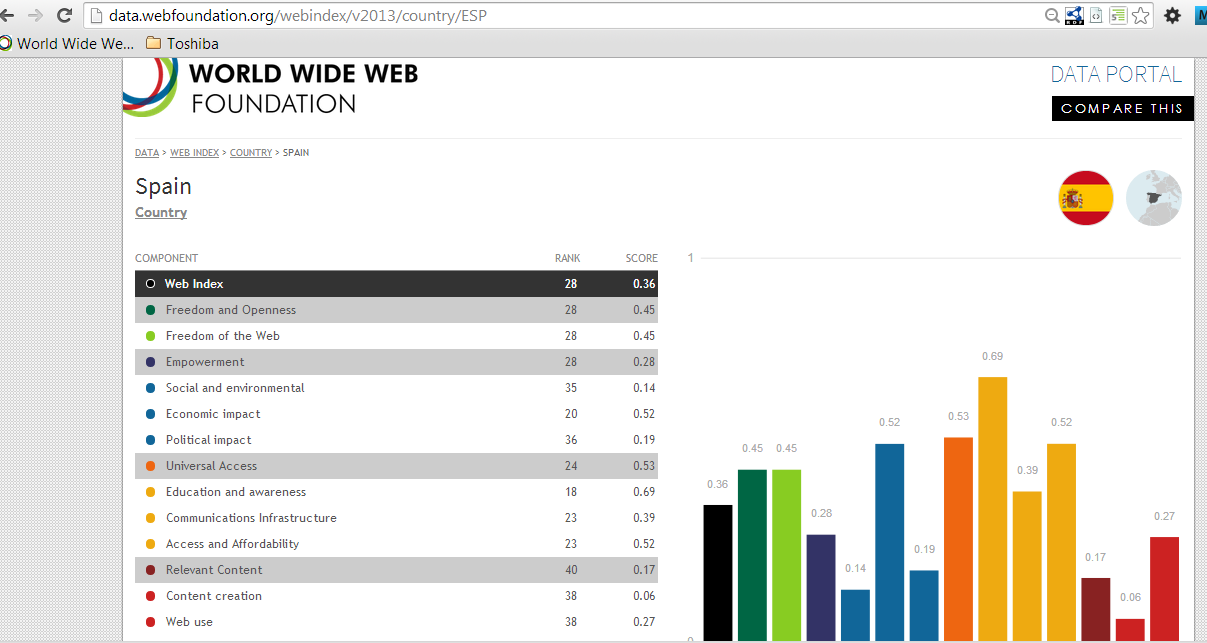
\includegraphics[width=0.9\textwidth]{WebIndexSpain}
\end{center}
\caption{Web Index visualization of country Spain}
\label{Fig:WebIndexSpain}
\end{figure*}

When there is no template for a given type of node, Wesby shows a table of properties and values similar to Pubby. For example, figure~\ref{Fig:WebIndexWeightMap}

\begin{figure*}[h]
\begin{center}
  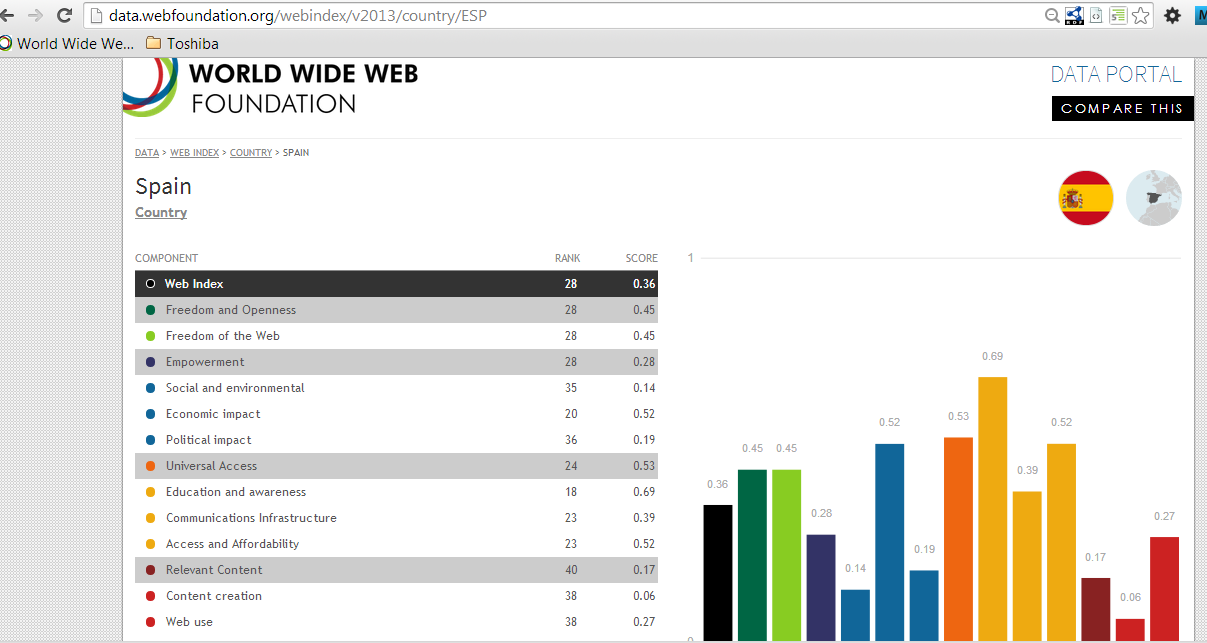
\includegraphics[width=0.9\textwidth]{WebIndexSpain}
\end{center}
\caption{Web Index visualization of a weight map}
\label{Fig:WebIndexWeightMap}
\end{figure*}
  
\section{Related work}

There is a growing interest in developing solutions to improve the quality of linked data~\cite{hogan10,Mendes12,kontokostasDatabugger}. 
We consider that is is very important to publish linked data that is not only of high
 quality, but also that can automatically be validated. 
 Validating RDF has also attracted a number of approaches. 
 Most of them were presented at the W3c Workshop on RDF Validation~\cite{RDFValidation} and can
be summarized as: 

Inference based approaches which try to adapt
RDF Schema or OWL. However, the use of Open World and Non-unique name assumption limits the
validation possibilities. \cite{ClarkSirin13,Tiao10,Motik07} propose the use of OWL expressions with a Closed World Assumption to express integrity constraints. 

SPARQL queries can express the validation constraints. SPARQL has much more expressiveness than Shape Expressions and was proposed in~\cite{Labra13} to validate the WebIndex before it was generated. 
After the WebIndex has been launched we noticed that validating the whole WebIndex data portal using the
SPARQL approach was not efficient so we have been involved in the development of Shape Expressions. 

Grammar based approaches define a domain specific language to declare the validation rules. 
OSLC Resource Shapes~\cite{OSLCResourceShapes} 
have been proposed as a high level and declarative description of the expected contents of an RDF graph expressing constraints
on RDF terms. Dublic Core Application Profiles~\cite{KarenCoyleTomBaker13} also define a set of validation constraints using Description Templates. Finally, Shape Expressions have been proposed as another technology inspired by RelaxNG~\cite{RelaxNG} and based on regular bag expresions~\cite{Boneva2014}.

Representing statistical linked data has also seen an increasing interest. 
SDMX~\footnote{\url{http://sdmx.org/}} is the primary format of the main statistical data organizations. In~\cite{Capadisli13} describes a the transformation of SDMX-ML data to RDF/XML. 
The RDF Data Cube vocabulary~\cite{Cube} has been accepted as a W3c Recommendation technology to publish multi-dimensional statistical data and to link it with other concepts and data. 
We have opted to follow the RDF Data Cube vocabulary and in fact, we consider that Computex can be seen as a further specialization of RDF Data Cube to represent statistical index computations.

Another piece of related work is how to represent mathematical expressions in RDF. 
Lange~\cite{Lange13} gives an overview of the different approaches. 
OpenMath was proposed as an extensible standard that can represent the semantic meaning of mathematical objects. 
Wenzel and Reinhardt~\cite{Wenzel12} 
propose an approach to integrate OpenMath with
RDF data for the representation of mathematical relationships and the integration
of mathematical computations into reasoning systems.

\section{Conclusions}

In this paper, we described how we were able to represent statistical index computations as linked data which include information to track the origin of any published observation.

Although the number of triples were around 3 million, we consider that the data portal is of medium size, so we were able to play with different validation possibilities.
In fact, although we initially wanted to do the whole computation process using SPARQL CONSTRUCT queries, we found that it took longer than expected (around 15 minutes for a subset of the whole dataset) so we opted to develop an independent Scala program in Scala that did all the computation in a few seconds.

After participating in the W3c RDF Validation workshop we were attracted by the Shape Expressions formalism. We developed the documentation of the data portal using Shape Expressions and we have developed an RDF validation tool using it. We consider that some structural parts of the data portal can be better expressed in Shape Expressions, while the computational parts could be expressed using Shape Expression semantic actions, all of which could be finally translated to SPARQL.

Using SPARQL queries to validate and compute index data seems a promising use
case for linked data applications. 
Although we have successfully employed this approach to validate most of the
statistical computations we needed for the WebIndex project, we have found some
limitations in current SPARQL 1.1 expressivity with regards to built-in
functions on maths, strings and RDF Collections.

Our future work is to automate the declarative computation of index data
 from the raw observations and to check the performance using
 the Web Index data. 
We are also studying the feasibility of this approach 
 for online calculation of index scores and rankings. 
% \TODO{Visualization of computed values?}

\section{Acknowledgements}

We would like to thank Jules Clements, Karin Alexander, César Luis Alvargonzález and Ignacio Fuertes Bernardo for their collaboration in the development of the WebIndex project.

\bibliographystyle{abbrv}
\bibliography{computex}

\end{document}
